\documentclass{article}
\usepackage{graphicx}
\usepackage[backend=biber,style=authoryear]{biblatex}
\addbibresource{My Library.bib}

\title{Literature review}
% General introduction on the forest managemet problem, the scale issue and the model question. Literature overview and research gaps for the development of new frameworks for forest management.

\begin{document}

\maketitle

\tableofcontents

\newpage

\begin{abstract}
    This literature review explores the forest management problem, scaling challenges, and the role of models, identifying limitations in current methods and highlighting research gaps. Forest management is evolving to address the dual challenges of climate change and new objectives for forest ecosystems. It is a complex, multidimensional problem that demands sustainable solutions across extensive spatial and temporal scales.
    
    Scale presents a significant challenge, affecting the patterns and interrelationships of ecosystem services, timber production, economic factors, and ecosystem equilibrium. Process-based models serve as crucial tools to address these scaling issues, offering quantitative insights into ecosystem processes and predicting multi-scale emergent functions. These models are increasingly utilized in forest management planning and decision-making but their complexity limits the use of traditional optimization methods.
    
    Key research gaps include (1) insufficient integration of social systems in forest management, (2) challenges in incorporating uncertainty, (2) difficulties in multi-scale ecosystem analysis, and (3) the need for a novel approach that combines ecological process-based models with the mathematical flexibility of viability theory.
    
    To conclude this review, we propose to work on bridging the gap between optimization and comparison approaches, integrating process-based models with mathematical tools to provide a range of possible solutions for forest management. This framework aims to develop decision support tools that address the multi-scale complexity of forest ecosystems and provide sustainable strategies for decision makers.
\end{abstract}

\newpage

\section{Introduction}

The history of forest management \\
Climate change and the future of forests \\
New objectives for forest ecosystems : FES, adaptative forest management \cite{yousefpourFrameworkModelingAdaptive2017} : framework for choice but limits in knowledge or DSS model uncertainty and behavioral aspect of decision making. \\ %calls for new tools inside the framework

Questions :
\begin{itemize}
    \item How to plan management at forest scale in the face of climate change and new objectives?
    \item What are the challenges of scale in forest management and how can they be addressed?
    \item What role do models play in understanding and managing forest ecosystems?
    \item What are the limitations of current methods and what research gaps need to be addressed to develop new frameworks for forest management ?
\end{itemize}

\section{Scales, organisation and processes in forest ecosystems}

\subsection{Scale in ecology}

The question of scale became prominent in ecology during the 1980s. \textcite{wiensSpatialScalingEcology1989} and \textcite{levinProblemPatternScale1992} were among the first to emphasize its importance. While scale had already been a significant topic in other fields such as geography, sociology, and economics, it had not been thoroughly explored in ecology due to practical experimental reasons, historical context, and researchers bias (\cite{wiensSpatialScalingEcology1989}). Researchers called for the development of a 'science of scale' in ecology, where scale would be an explicitly stated variable in analyses (Meentemeyer \& Box, 1987). Some went further demanding the development of scaling theory, making it a central focus of ecological research (\cite{wiensSpatialScalingEcology1989}). Key characteristics of scale, such as grain and extent, were highlighted (\cite{wiensSpatialScalingEcology1989}), along with aggregation issues in parallel works (\cite{gardnerRobustAnalysisAggregation1982}). \\

Hobs reminds the twofold of this problem : the "big scale" (estend or range) and "small scale" (grain or resolution) problem [need to define ?] and summarizes some problems and challenges offered by scale to ecologist in a paper [Hobbs 2002] :
\begin{itemize}
    \item Ecologist observe a small part of the world
    \item The scale affect what is observed
    \item Heterogeneity is often the rule
    \item Large scale studies are not the silver bullet
    \item The scale of human knowledge limits the one of their actions
\end{itemize}

Twenty years after the first questions on scale, there was still significant progress to be made. In a review of 79 multi-scale wildlife habitat studies published since 1993, \textcite{wheatleyFactorsLimitingOur2009} found that 70\% of the observational scales were chosen arbitrarily.

\cite{chaveProblemPatternScale2013} : The problem of pattern and scale in ecology: what have we learned in 20 years? : extract infos \\

Exemple of scale in one specific ecosystem property : biodiversity ?? \\

The work of \textcite{vellendGlobalMetaanalysisReveals2013} also highlights the critical issue of scale in ecological research. The debate (\cite{gonzalezScalingupBiodiversityecosystemFunctioning2020}, Cardinale 2018) that followed this publication revealed that the challenge of reconciling findings from studies conducted at different spatial scales was still not solved. In his global meta-analysis, Vellend concluded that there was no net change in local-scale plant biodiversity over time, based on aggregated data from multiple localized experimental studies. This finding appears to contradict the broader narrative of global biodiversity loss driven by habitat destruction, climate change, and other large-scale anthropogenic impacts. However, these conclusions are not contradictory but rather underscore the importance of scale in interpreting ecological data. The absence of net biodiversity change at local scales does not mean that global biodiversity is not declining. Instead, it reveals that local and global biodiversity patterns are governed by different processes, requiring careful interpretation to avoid conflating scales and questioning the relevance of local studies in addressing global biodiversity loss issues.

\begin{figure}[h]
    \centering
    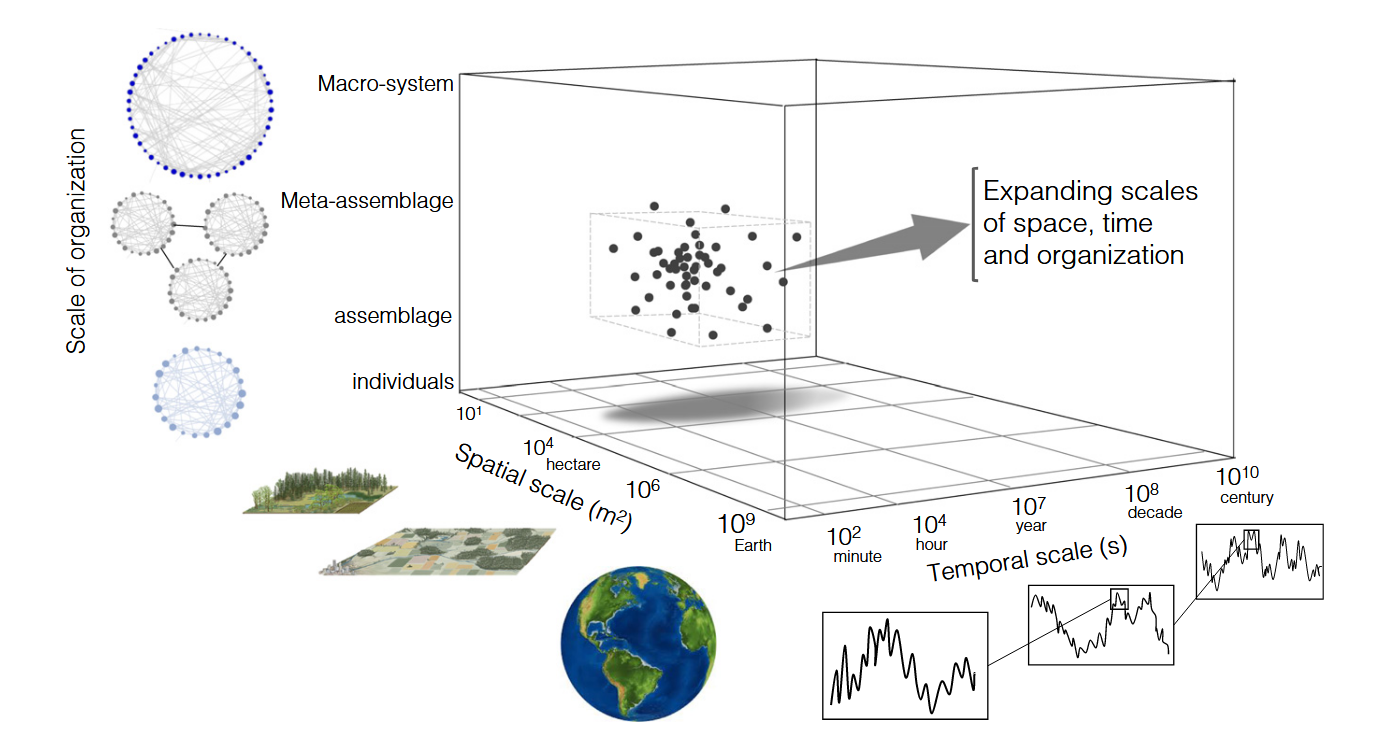
\includegraphics[width=\textwidth]{images/BEF_scales_Gonzales.png}
    \caption{Scales of BEF studies (\cite{gonzalezScalingupBiodiversityecosystemFunctioning2020})}
    \label{fig:BEF_scales}
\end{figure}

The challenge of upscaling persists as we confront global issues constrained by experimental limitations \cite[see Fig. \ref{fig:BEF_scales}]{gonzalezScalingupBiodiversityecosystemFunctioning2020}. \textcite{gonzalezScalingupBiodiversityecosystemFunctioning2020} examine both theoretical and empirical evidence, highlighting the non-linear nature of biodiversity-ecosystem functioning (BEF) relationships across different scales. They emphasize the necessity of employing various biodiversity metrics to fully capture these dynamics. Specifically: (1) Alpha diversity refers to the species diversity within a particular area or ecosystem, often measured by the number of species (species richness) in that area. (2) Beta diversity measures the change in species composition between different ecosystems or areas, indicating the turnover of species across space. (3) Gamma diversity is the total species diversity within a large region or landscape, combining both the alpha diversity of individual ecosystems and the beta diversity among them.

This research (\cite{gonzalezScalingupBiodiversityecosystemFunctioning2020} REF in Gonzales ?) underscores the ongoing importance of understanding how grain, extent, and aggregation influence ecosystem processe, particularly given the complex and non-linear scaling laws that remain inadequately defined in current biodiversity and ecosystem research.

And also the temporal scale effect (Gonzales 2000). \\

To the non linarity problem Bugmann underline two other properties of upscaling or downscaling (Bugmann 2000): (1) Hierarchical systems (new level of organisation and interaction between each) (2) Spatially heterogeneous (No representativity between scales). 
\cite{messierDealingNonlinearityUncertainty2016} non-linearity and uncertainty in forest. \\

\textcite{seidlScalingIssuesForest2013} reachs the same conclusions for forest ecosystem : if the theory of scaling in ecosystems exist its diffusion in the field is limited. However it is significant for multiple reason :
\begin{itemize}
    \item Choice of the processes to implement
    \item Impact of climate change on those different processes (CO2 at the scale of cell metabolism, dsturbance at the landscape scale)
    \item hierarchie and emergent processes : additive properties by changing scales but also non linear properties or new concepts/caracteristics that did not exist in the lower scale (like the concept of patch in landscape ecology, or biodiversity when going from species dynamics to community or ecosystem)
\end{itemize}

\subsection{Application to forest ecosystems}

\subsubsection{Exemple of the scaling problem in forest ecosystems}

The scaling problem has been shown to significantly impact forest ecosystems. Both experimental and modeling studies indicate that the spatial level of analysis influences the observed patterns of ecosystem service (ES) supply and their interrelationships. On the experimental side, chisholm 2013 examined the effect of tree species richness on forest biomass and productivity across 25 forest plots, varying the spatial grain from 0.04 to 1 hectare. Their findings revealed that grain size qualitatively alters the relationship between tree diversity and productivity metrics, such as above-ground biomass and coarse woody debris production. The influence of spatial scale on ecosystem service patterns is further illustrated by \textcite{roces-diazSpatialLevelAnalysis2018} (see Fig. \ref{fig:Spatial_pattern_RocesDiaz}), who demonstrated that changes in spatial resolution not only modify these patterns but also affect trade-offs between ecosystem services and biodiversity, underscoring the need for careful consideration when analyzing such relationships. Moreover, \textcite{schallImpactEvenagedUnevenaged2018} showed that varying the scale of analysis impacts biodiversity indicators beyond tree species, noting that conclusions about the effects of uneven-aged forest management can differ markedly between alpha and gamma diversity for certain taxa.

\begin{figure}[h]
    \centering
    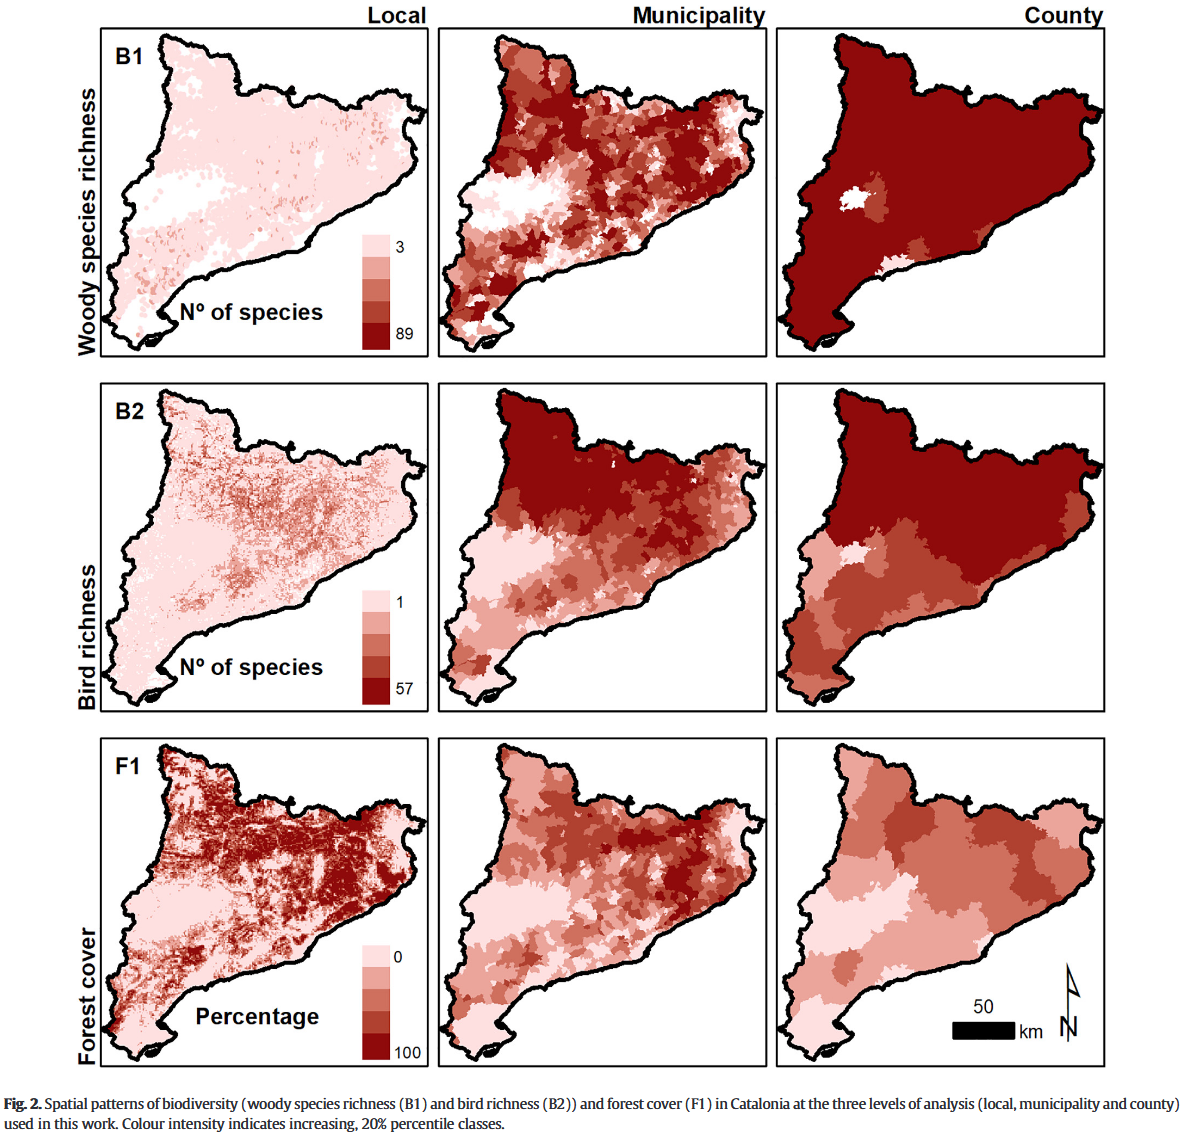
\includegraphics[width=\textwidth]{images/Spatial_pattern_RocesDiaz.png}
    \caption{Spatial pattern of forest ecosystem services supply and their relationships \cite{roces-diazSpatialLevelAnalysis2018}}
    \label{fig:Spatial_pattern_RocesDiaz}
\end{figure}

Modeling studies reveal similar patterns, demonstrating that the spatial resolution can significantly influence the dynamics and interpretations of forest ecosystems. Varying the resolution can lead to different outcomes in simulated forest structures over time. For example, \textcite{smithScaleResolutionForest1988} showed that simulating a 9-hectare forest stand with different grid resolutions produced varying forest structures. Larger quadrats tended to suggest a stable equilibrium, whereas smaller quadrats revealed more dynamic and fluctuating structures. This highlights the importance of selecting an appropriate spatial resolution in forest modeling to avoid misinterpretations of ecosystem dynamics.

\subsubsection{Scale, level of organisation and processes}

In forest we can describe different scales and levels of organisation. They may be consistent, but the scales of observation are not always the same as the scales of organisation. In forest the main observed scales are : tree, stand, landscape, regional, global. They actually describe level of organisation for different reasons : the tree scale is the ecological level of organisation of an organism while the stand scale is deffined as a management unit and may not be an ecological level of organisation. However social organisation is also important in forest management and the stakeholding level might need to be added to understand the ability of management to change in the future in order to keep the forest sustainable. Scales and level of organisation that are found in forest studies are described in Fig \ref{fig:Scales_levels_forest}, in the following I will use the geographical scale to describe the different scale of my study but it is iomporrtant to keep in mind the new level of organisation they encompass when taking them into account. \\

Upscaling then becomes a question of the new processes and interaction that need to be taken into account when changing the scale of observation. New processes arise at the scale of forests, such as disturbances (fire, pests), population dynamics (animal species), seed dispersal, and water flow. These processes are not observable at the tree scale but become significant at the forest scale, influencing the dynamics and equilibrium of forest ecosystemsb [DETAILS]. Moreover, the addition of spatial organization questions, such as patch size, shape, adjacency, and corridors for different species, further complicates the scaling problem in forest ecosystems \cite{baskentSpatialForestPlanning2005}. \\

\subsection{Social system, governance and forest management}

see fischer 2018

Often neglected in the literature (seen in limits multiple times), but the social system is a key component of the forest management problem. \\
\cite{mannAssessingForestGovernance2021}
\cite{keenanClimateChangeImpacts2015}: the limit in research is not uncertainty or knowledge but the communication with community and decision makers. Adaptation is a social process.
\cite{vacikCurrentFutureDrivers2014}: emerging features of DSS mainly accessibility through internet, visualization tools, 

In forest 
Socio-ecological systems
Limits \cite{artsForestsPolicyAnalysis2012}

\subsection{Consequences for management, opportunity and complexity}

The scale of forest studies is also central in forest management contexts, where it influences timber production flows and economic dynamics. Achieving equilibrium in forest ecosystems requires a focus on larger spatial and temporal scales.

Ignoring landscape-scale processes can lead to errors in forest management. Approaches focusing on stand-level management have lead to undesirable landscape conditions and increased vulnerability to disturbances \cite{Hunter1990,Cissel1994,Bergeron1999}. For instance, uneven forest management, which has shown positive outcomes at the stand level—particularly in terms of enhancing alpha biodiversity (REF) — can result in the loss of gamma diversity when applied at a larger spatial scale. This occurs due to the homogenization of habitats and a reduction in landscape heterogeneity \cite{heinrichsLandscapeScaleMixturesTree2019}. These findings highlight that maximizing individual forest functions at the stand scale may not necessarily translate into optimal landscape-scale outcomes.

Then particular attention should be paid to the choice of the right scale for minimizing trade-offs between different management goals. For exemple the trade-offs between timber production and carbon storage can be less severe and more effectively mitigated at larger planning scales \cite{pohjanmiesMoreMoreForest2017}. This not only has ecological implications but also offers a pathway to reduce conflicts and minimize disagreements among ressource users, thus enhancing the effectiveness of management strategies.

Several hypotheses suggest that a diversified management approach at the landscape scale can enhance biodiversity. For example, \cite{duflotManagementDiversityBegets2022} propose five key hypotheses: (1) \textit{The Habitat Diversity Hypothesis}, where greater management diversity increases landscape-scale beta species diversity; (2) \textit{The Spatio-Temporal Heterogeneity Hypothesis}, which suggests that asynchrony in management timing enhances the long-term availability of different habitat types; (3) \textit{The Interspersion Hypothesis}, which emphasizes the importance of spatial adjacency or proximity between stands with different management or successional stages for increasing biodiversity; (4) \textit{The Natural Forest Hypothesis}, which argues that heterogeneous unmanaged set-aside forests are necessary for complete biodiversity conservation; and (5) \textit{The Temporary Corridor Hypothesis}, which posits that management diversity creates temporary connections between protected forests for multiple species. These hypotheses can be tested through simulations or thought experiments, and provide valuable insights into how landscape-scale management diversity can foster biodiversity in production forest landscapes.

\begin{figure}[h]
    \centering
    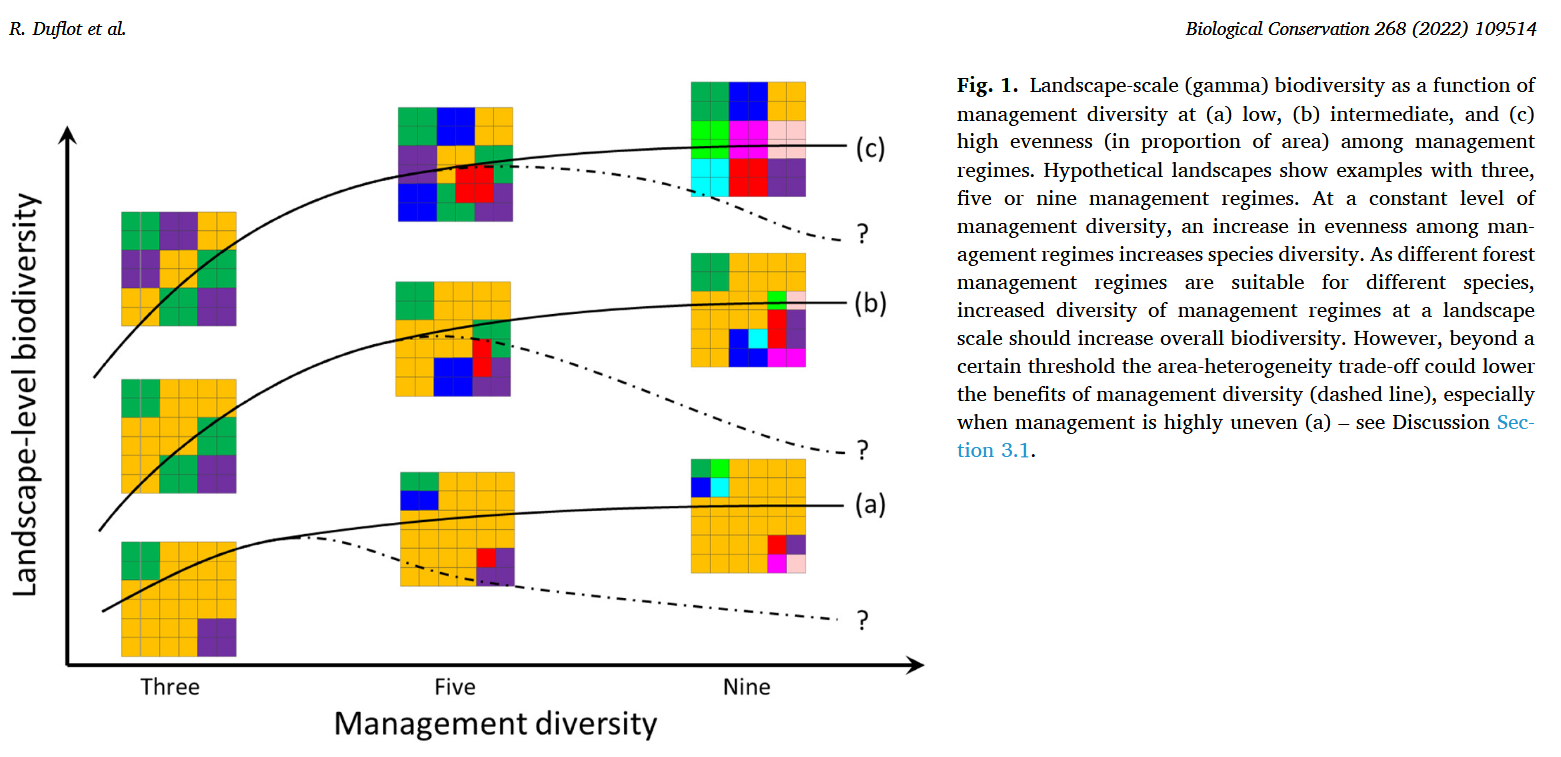
\includegraphics[width=\textwidth]{images/Management_diversity_Duflot.png}
    \caption{Management diversity hypotheses \cite{duflotManagementDiversityBegets2022}}
    \label{fig:Management_diversity}
\end{figure}

Hypothesis (2) was tested in agricultural system in the thesis of \cite{Sabatier2020}. The focus of his work lies in explicitly addressing the trade-offs between various management goals, and in particular, understanding how the spatial arrangement of land uses effects on ecological and productive performance at the landscape scale \ref{fig:Spatial_structure}. Sabatier's research suggests that playing with the spatial arrangement of management strategies within the landscape provides an opportunity to mitigate conflicts between competing objectives. This approach could also be relevant for forest management, where spatial structuring of various management types has the potential to improve landscape-level sustainability. 

In fact, the concept of using spatialization to optimize functionality has already been explored in forests. For instance, \cite{garcia-quijanoScalingStandLandscape2008} illustrates how the spatial arrangement of management strategies at the stand scale can improve forest carbon sequestration at the landscape scale. According to \cite{Seidl2013}, scaling in forest management can assist managers in four key areas: (1) avoiding misinterpretations of new data by ensuring that the associated scale and context are understood; (2) minimizing scaling errors and reducing uncertainty; (3) improving the integration of multiple ecosystem services; and (4) enabling the integration of novel management strategies.

\begin{figure}[h]
    \centering
    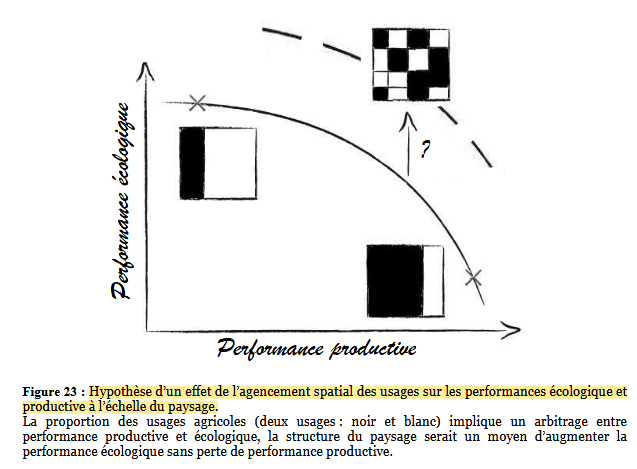
\includegraphics[width=\textwidth]{images/Spatial_structure_Sabatier.png}
    \caption{Spatial structure in landscape management \cite{Sabatier2020}}
    \label{fig:Spatial_structure}
\end{figure}

However, studying forest at this scale also presents challenges. Scaling up forest management introduces additional problems that must be solved. To the question of which management (the tactical decisions regarding specific actions to be taken) to implement in each location is added the question of where (strategic location of management activities) to implement these management actions, taking into account spatial arrangement, interaction, and heterogeneity of the landscape \cite{Bos1993, Povak2024}. The challenge lies in resolving these issues simultaneously, as solving one often impacts the other \cite{Baskent2005}.

Thus, while landscape-scale forest management is fraught with complexity, it also presents a unique opportunity to align forest management with the broader ecological and socio-economic goals of sustainability, resilience, and multifunctionality.

\section{Solving the management problem, philosophy and tools}

\subsection{Models for forest management}

simulation models [DEFINITION] are great to tackle those questions of scale for 2 main reasons \cite{seidlScalingIssuesForest2013} : (1) conceptualisation of ecosystem functionning giving quantitative output of those processes (2) predictions and multi-scale emergent functions. \\
\cite{wolfslehnerHarnessingEcosystemModels2010} : they are increasingly applied in the context of forest management planning and decision support in particular coupled with MCDA (Multi-Criteria Decision Analysis).

However there is a lot of different models and simulation or processbased model are only a small part of it. To review the litterature on the subject read \cite{pretzschModelsForestEcosystem2007} and \cite{shifleyFutureModelingForest2017}. In order to study large scale ecosystem the focus of my wok is on landscape model that have also been extensively reviewed and clasified \cite{heForestLandscapeModels2008} and \cite{xiReviewForestLandscape2009} as wee as \cite{schellerEcologicalClassificationForest2007}. \\

Not going to come back on the specificity of each models but maybe a classification can be interesting and an exemple of processes generally inclueded (in two figures). Also the fact that even though they have been a work to classify the different types of models there is still no uniformity in the litterature to describe them. \\

Scale in models : \textcite{seidlScalingIssuesForest2013} The choice of scales in models is crucial, particularly in representing landscape heterogeneity and the emergence of specific patterns. It is essential to select an appropriate resolution to accurately capture these dynamics and ensure the validity of the model's predictions.

Not only the scale chosen but the method of upscaling (implicitor explicit (Extrapolation by lumping, direct extrapolation, extrapolation by expected value, extraplation by analytical integration)) can change the results : \cite{bugmannScalingIssuesForest2000} (Figure \ref{fig:Spatial_pattern_Bugmann}). Detail about those methods can be found in this article or in King 1991. [ICI OU DANS Scale in forest]

\begin{figure}[h]
    \centering
    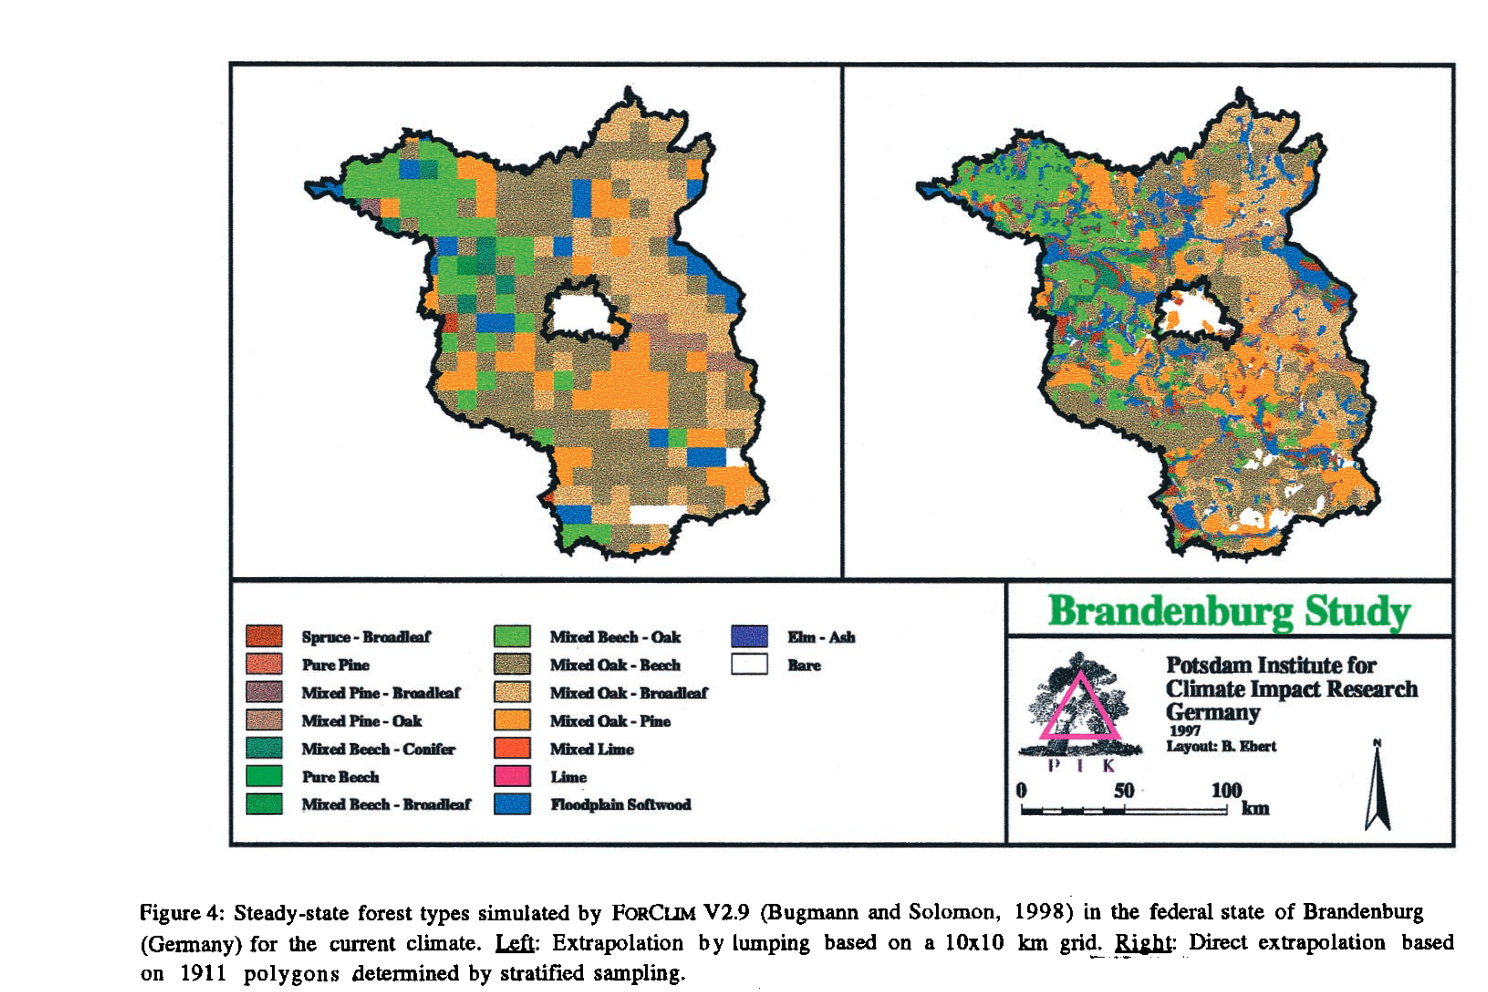
\includegraphics[width=\textwidth]{images/Spatial_pattern_Bugmann.png}
    \caption{Pas necessaire ? Spatial pattern of forest ecosystem services supply and their relationships \cite{bugmannScalingIssuesForest2000}}
    \label{fig:Spatial_pattern_Bugmann}
\end{figure}

There are two main approaches in the literature to solve the management problem: (1) the optimization approach, which aims to find the best solution to a given problem, and (2) the comparison and evaluation approach, which aims to evaluate and compare a priori defined strategies to meet the objectives of the problem. \\

\subsection{Optimization}

Two reviews on the subject from 2016 and 2025. How are management problem fomulated and solved, what are the limits of such approaches. \\

Optimization in forest management \cite{kayaOptimisationForestManagement2016}
Cite multiple other reviews on the subject
Give an overview of the methods used to solve the problem (difference between optimization, heuristic, linear programming...)
Many of the issues facing forest-level management planning today are spatial in nature.
The constraints used at the forest level involved area control, wood flow (minimum, maximum, periodic fluctuation, even-flow, etc.), harvest area (opening) sizes, adjacency of harvests, sizes of core (older forest) areas, minimum harvest ages, ending standing inventory levels and others that relate to maintaining biodiversity or wildlife habitat, producing non-timber forest products, and providing recreational experiences.
Area where research is needed \cite{kayaOptimisationForestManagement2016}: concepts that may be difficult to quantify, such as ecological health or resiliency, and how these can be integrated into optimization methods. multi-objective optimization is difficult in many respects, particularly when the relationships between decisions and outcomes are non-linear or when the decisions are binary (or simply integer)

\cite{labarreImprovingForestDecisionmaking2025} : Review on decision making tools in forestry including (optimisation stochastic methods, robustness and viability). With an emphasize on uncertainty or climate change as well as a comparison to viability theory. From a first search with a thousand article they selected 100.
Main conclusions :
\begin{itemize}
    \item Quantitative approachs integrating uncertainty and complex system theory into forest management planning mainly comes from operations research, economics and finance. (see Fig. \ref{fig:Decision_tools_labarre})
    \item Viability is rare (6 articles) but it could be a way to integrate process-based descriptive models.. interesting (comparison with the other methods)
    \item Limit of optimality : 
    \item 
\end{itemize}

\begin{figure}[h]
    \centering
    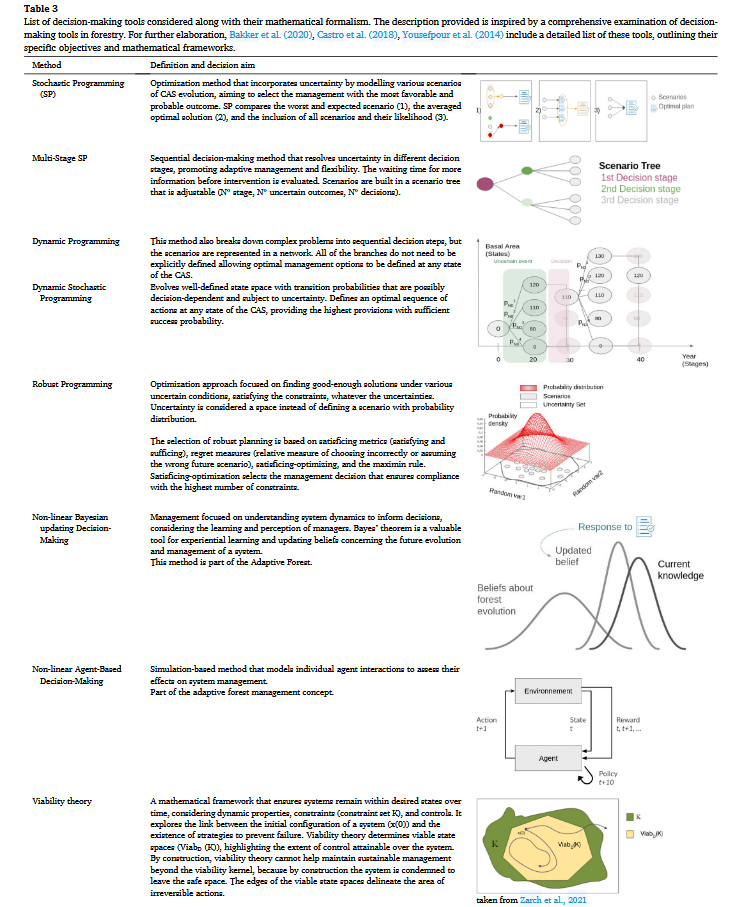
\includegraphics[width=\textwidth]{images/Decision_tools_labarre.png}
    \caption{Decision tools in forest management \cite{labarreImprovingForestDecisionmaking2025}}
    \label{fig:Decision_tools_labarre}
\end{figure}

Link between forest model and mathematical heuristics : \cite{labarreImprovingForestDecisionmaking2025} (see ) \cite{vacikCurrentFutureDrivers2014}: Over the recent decade, forest growth models have been used in combination with optimization and choice algorithms to support forest planning. [ MAIS JE NE SAIS PAS OU NI QUOI, A creuser]

\begin{figure}[h]
    \centering
    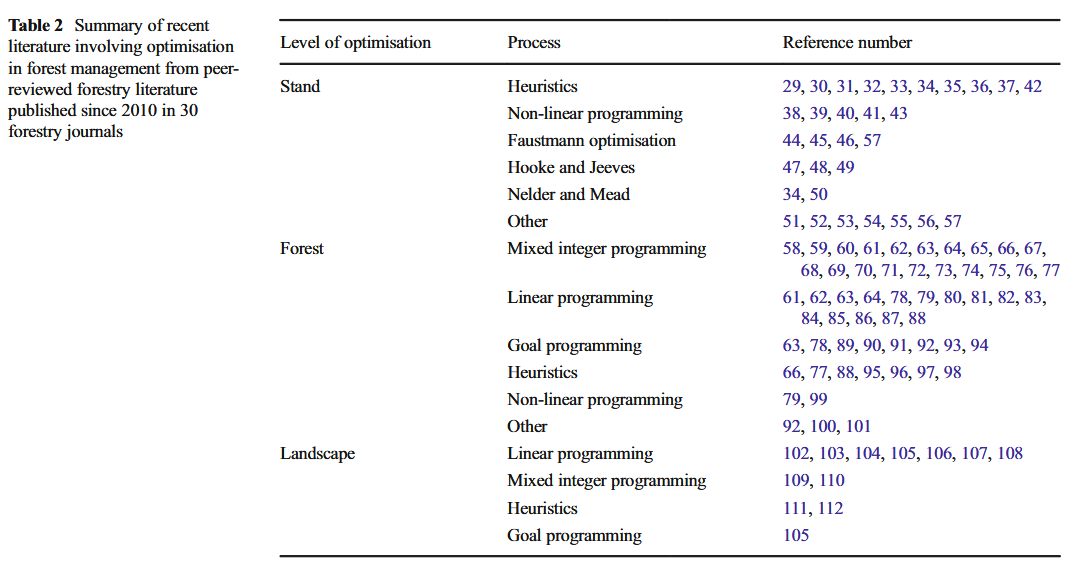
\includegraphics[width=\textwidth]{images/Optimisation_methods_Kaya.png}
    \caption{Optimization methods in forest management \cite{kayaOptimisationForestManagement2016}}
    \label{fig:Optimisation_methods}
\end{figure}

\cite{bettingerKeyLiteratureTrends2004}: The key literature of, and trends in, forest-level management planning in North America. linear programming to heuristics methods. Main goal being economics and wood production. Mainly applying mathematical advances in other fields to this problem. \\

Journals in which those articles are published \\
Kind of tools used: (1) linear programming (2) dynamic programming (3) heuristic methods (4) simulation-optimization models (5) Lagrangean relaxation \cite{andalaftProblemForestHarvesting2003}, planning problem road and maintenance \\

\cite{bosZoningForestManagement1993} formulating the zoning problem as a quadratic assignment. zoning research is scarce because large problems are difficult to solve with linear programming. [In here or in scale]\\

\cite{crowleyUsingEquilibriumPolicy2014}: Using Equilibrium Policy Gradients for Spatiotemporal Planning in Forest Ecosystem Management

Type of models: 

Mainly focusing on rotation age
Limits: behaviors, spatial interactions, risk, uncertainty (The forest harvesting problem: have we reached the limit of our understanding? \cite{amacherForestHarvestingProblem2015}) \\

\subsection{Comparison and evaluation}

Journals in which those articles are published \\
Large literature in different systems (boreal, tropical, temperate), different objectives (carbon, biodiversity, timber, water, fire, pests), different strategies tested (even-aged, natural regeneration, clearcutting, selection cutting, salvage logging, prescribed burning, pest control, assisted migration), different models (FVS, LANDIS, SORTIE, iLand, CRAFTY, FORMIND, 3-PG). \\
Advantages: (1) processes (emergent dynamic) (2) more operational (3) climate change

\cite{duveneckEffectsAlternativeForest2014}: archetype of this type of article (highlights the limits: climate uncertainty, ecological uncertainty, ecological process missing, lack of social interaction with the ecosystem) \\

My questions ? Can they be answered by the kind of study I did ? \\
Integration and interaction of different scales \\
Management scale and spatialisation \\

\section{Limits and possible question for my research}

\subsection{Meeting halfway or the need for a new approach}

Clear separation between the two approaches. (1) Maybe because it comes from different fields (economics, ecology, engineering). (2) But also because of the complexity problem. [Maybe a link between both in DSS literature see \cite{vacikCurrentFutureDrivers2014}] \\
But they share the same philosophy: one right way to manage the forest. Maybe there is another solution to the problem. \\
Linking the two approaches by using mathematical tools with ecological process-based model and using an approach that could give a range of possible solutions rather than one optimal one. \\
Viability theory (Aubin 1991) \\
Use of viability theory in forest \cite{mathiasUsingViabilityTheory2015, mathiasMultilevelPoliciesAdaptive2017, pichancourtBridgingOstromsGovernance2024}

\subsection{Multiscale decision support tools}

\subsection{Other limits in the literature}
That we might need to work with, for which other research could be interesting. \\
uncertainty (body of research on this): \cite{radkeIdentifyingDecisionrelevantUncertainties2020}: Approaches that analyze decisions under deep uncertainty include robust decision-making (Lempert et al. 2003), many objective robust decision-making (Kasprzyk et al. 2013), dynamic adaptive pathways (Haasnoot et al. 2013), adaptive policy-making (Hamarat et al. 2014), and direct policy search (e.g., Quinn et al. (2017)). \cite{depellegrinllorenteRecognizingUncertaintyForest2022} \\
Temporal scales \cite{chaveProblemPatternScale2013}
Land-use, no frontier in ecology (edge effect)

\section{Question, hypothesis, choice and objectives of this thesis}

\subsection{Question, hypothesis and objectives}

\subsection{Choice, tools and methodologic framework}

Forest model choice (comparaison Landis II, treemig, LandClim, iLand) \\
This model is integrated in a larger workflow, its limits need to be understood and taken into account in the interpretation of the results. But the goal of this thesis is to consolidate the framework in order to develop tools for strategies developpement and assessment. The model is one building block, it could be changed (with some limits) but the framework is the main goal. \\

\subsection{Constraints for systematic search}
Large field, defining some aspect, region, methods... (Horl 2020). Nb of article (quantitative)
Non-homogeneity of model classification

\printbibliography

\end{document}